% begin Chapter Introduction

\chapter{Introduction}
\label{chapter-Introduction}

\paragraph{ } The Private Bus Transportation System is a famously contentious topic in Sri Lanka. For the average commuter, complaining about the system is part and parcel of everyday life. As a commuter myself and having used public transportation extensively for more than a decade, I have wondered many a time about the reasons why the bus service is in this state and why people keep complaining about it so very vehemently. The constant complaints are justified, as the bus service is grossly inefficient and lack proper service quality. The inefficiency in the system leads to lost productivity and dissatisfaction by the commuters. Eventually, it is the country that suffers from the lack of an efficient public transportation system for the people.

The initial objective of my project was to pinpoint the existing problems and possibly provide an IT solution for them. During the course of the research and interviews with the numerous people involved with the public transportation sector, it occurred to me that the system has a myriad of things wrong with it. Careful management was the only requirement to overcome some problems, while others required a restructuring of the system, and still others required just an implementation of a solution and regulation of the service properly. Further research was required to identify underlying causes and provide a holistic solution to the problems. As I was passionate about the problem, I was intent on conducting a research to find solutions.

It is in this background that my research into the usage of an IT-based system to solve problems in the local public transportation service was carried out. I did not immediately arrive at a solution, but gradually understood that the problems and the requirements of the stakeholders demanded such a system. Consequently, I attempted to identify and abstract the system's key components so that the over-arching concept can be applied to similar transportation systems in other developing countries.

\section{Background Study: The Case of the \acrshort{wp} \acrshort{rpta}}
\label{section-BackgroundStudy}

\paragraph{ } Bus Passenger Transport is the highest and most widely used mode of public transport in Sri Lanka. The system is divided into Inter-Provincial and Intra-Provincial bus services. The service is operated by privately run (private buses) as well as state-run (\acrshort{sltb}) buses. The Sri Lanka Transport Board manages the \acrshort{sltb} buses and their jurisdiction is island wide regardless of the district or province. However, the organizational structure of private buses is different. All Inter-Provincial Private Buses are governed by the National Transport Commission (\acrshort{ntc}) while the private bus services within each of Sri Lanka's provinces are governed by the Passenger Transport Authorities of the respective provinces. Accordingly, the Western Province Road Passenger Transport Authority (\acrshort{wp} \acrshort{rpta}) handles the governance of the Private Bus Passenger Transport System in the Western Province. Please refer to Figure~\ref{image-busTransportSystemStructure} for an illustration of the Structure.

\begin {figure} [h!]
\centering
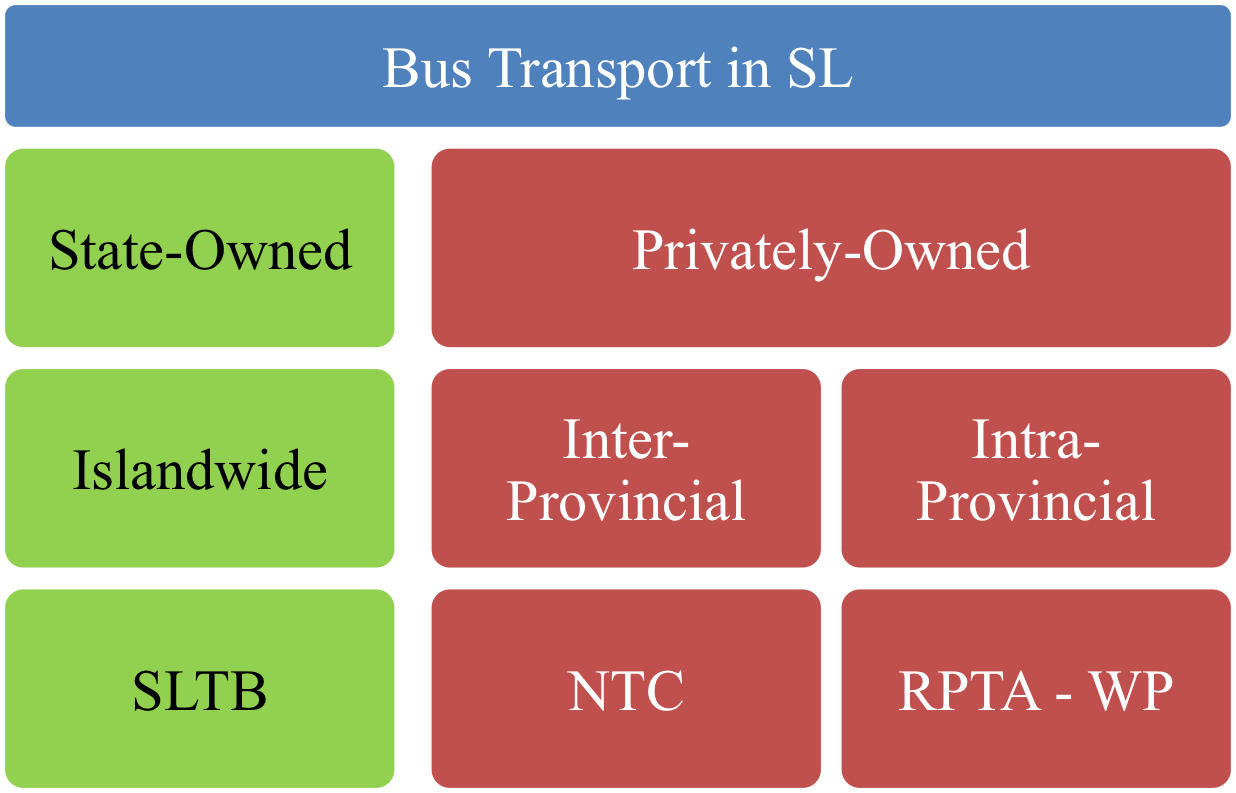
\includegraphics [scale=0.6] {busTransportSystemStructure}
\caption [Structure of the Bus Transport System in Sri Lanka] {The Structure of the Bus Transport System in Sri Lanka}
\label {image-busTransportSystemStructure}
\end {figure}

The major difference between the system in use in Sri Lanka and other countries is that the owners and operators of the buses are independent contractors and not the Central Government or the Provincial Authority. This has led to numerous problems and we shall discuss them in detail during the course of this document.

\subsection{Statistics of the Bus Service in Sri Lanka}

Let us take a look at some statistics involved with the bus service in Sri Lanka to fully grasp the magnitude of the system. According to the Draft National Policy on Transport in Sri Lanka \cite{MinistryofTransport2008}, public transport accounts for nearly 73\% of the total motorized passenger transport in the country. It also serves as the only means of transport for the majority of the population.

Of this, bus transportation accounts for nearly 68\% (a 93\% share in the public transport sphere), while rail transport accounts for the remaining 5\% (a 7\% share in the public transport sphere) \cite{MinistryofTransport2008}.

Within the bus transportation system, state-run bus services account for a 23\% share (about one-third of the share of bus transport) while private operators have a share of 45\% (a two-thirds share) provided by small-scale operators.

\begin {figure} [h!]
\centering
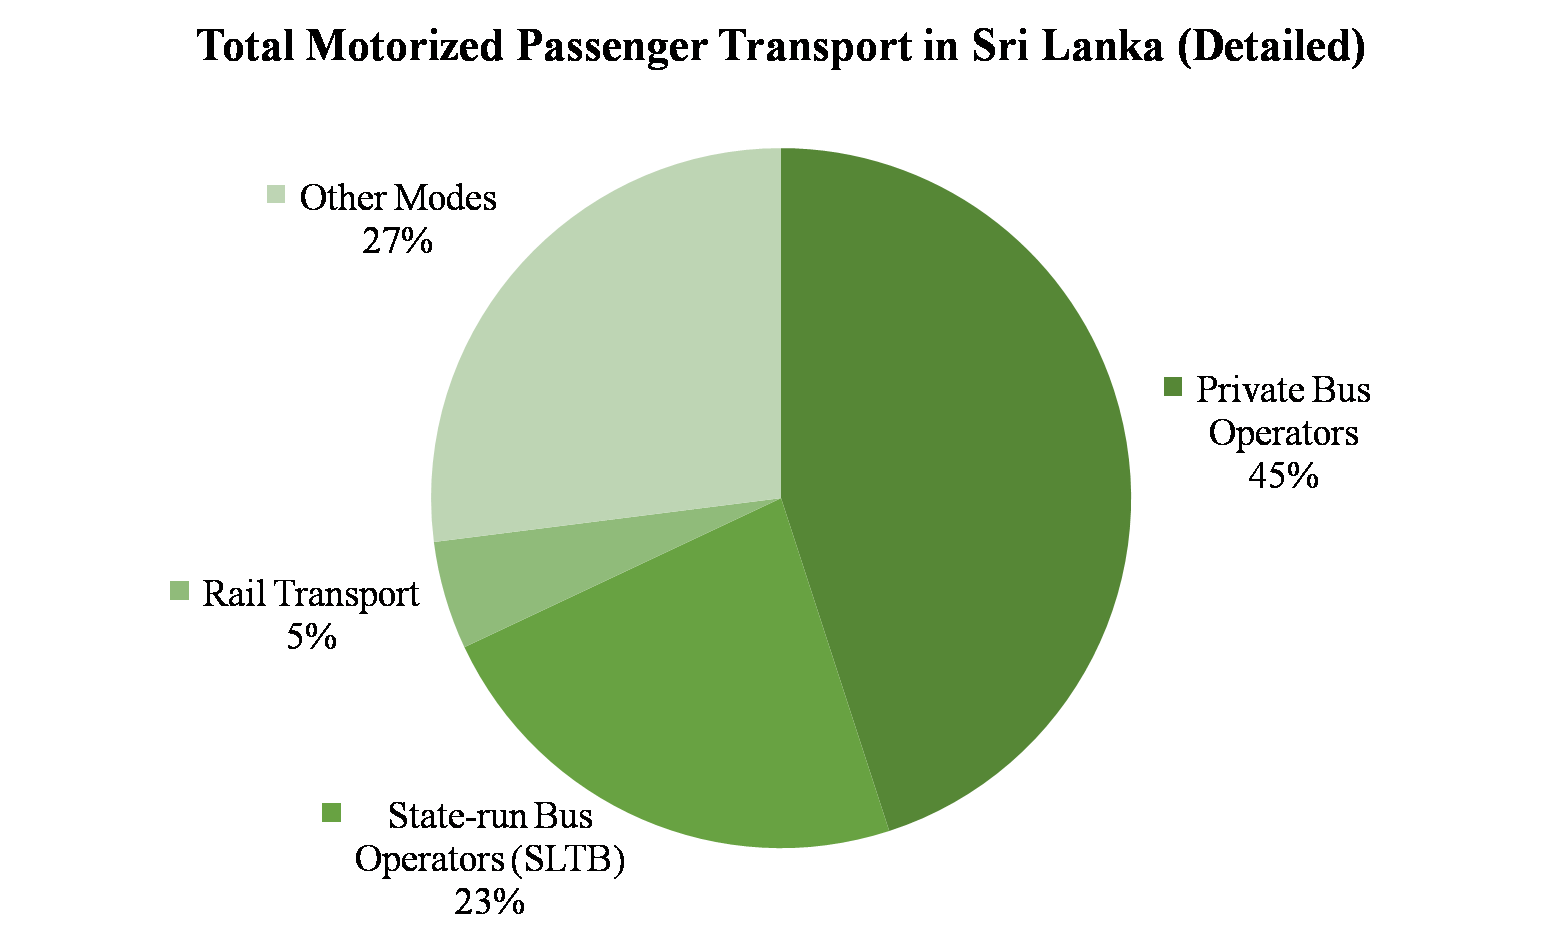
\includegraphics [scale=0.6] {totalMotorTransportPieChart}
\caption [Total Motorized Passenger Transport in SL] {Detailed View of Total Motorized Passenger Transport in Sri Lanka. Source: \cite{MinistryofTransport2008}}
\label {image-totalMotorTransportPieChart}
\end {figure}

Taking a look at the state-run bus service, data obtained from the Sri Lanka Transport Board show that approximately 2.5 million passengers island wide commute daily on close to 4500 \acrshort{sltb} buses \cite{SriLankaTransportBoard2010}. These buses travel an average of 2000km a day \cite{SriLankaTransportBoard2012}. 

Considering the buses operated by private bus operators, it is estimated that 10 million commuters travel daily on approximately 18,000 private buses currently in use in the country \cite{Silva2010}. Data gathered from the \acrshort{wp} \acrshort{rpta} show that there are around 7000 private buses servicing the Western Province and its' routes which is close to 450 in number. 

Looking at these statistics, we clearly see that the buses run by the private bus operators are far more in number compared to the state-run buses. It also shows that the majority of the commuters rely on the buses operated by private bus operators. These buses function as small independent operators and in 30 years of service operation, not even a single major private bus operator has emerged. The private bus "cartel" is highly unionized and dictates terms to the commuters as well as the government on a regular basis \cite{AdaDerana2012}. Bus strikes are very common and when they do happen, the commuters are placed in great discomfort \cite{Samarajiva2012, ColomboPage2012}.

In contrast, the state run bus service has a governing body, the SLTB, but it has been in steady decline since the 1970s owing to mismanagement and cost overruns \cite{AnswersDotCom2012}. It has now become a money-sucking state entity and continues to waste the tax payer's money with no solution on the horizon \cite{LBO2011, Sirimanne2013}. The number of SLTB buses in daily operation is well below the number of private buses and because of this, the state-run bus service is unreliable. Presently, it is but a teardrop in a sea of public transport dominated by the private bus operators. For example, as pointed out previously, there are more private buses in the western province (around 7000) than there are SLTB buses in the entire island (around 4500).Given that the average commuter cannot and does not wait for hours on end till an SLTB bus arrives, they have no other option but to use the private bus service. \cite{Wijayapala2012, Azwer2012}

\subsection{Justification of Research Project}

\paragraph{} As mentioned earlier, the Private Bus service is the largest and most widely used Passenger Transport system not only in the Western Province but also in Sri Lanka. However, commuters are constantly dissatisfied with the service provided and there seems to be no alternative. The railway system has its own problems and inefficiencies and a solution to that demands separate research.

According to World Bank statistics, Sri Lanka's population currently stands at 20.869 million people \cite{WorldBank2013}. Being the most densely populated, the Western Province has a population of 5.8 million people \cite{DepartmentofCensusandStatistics2012}, which is 27.8\% of the total population. This means that more than a quarter of the people in Sri Lanka live and commute in the Western Province. Therefore, it is clearly evident that an improvement in the level of service is needed seeing as it affects more than a quarter of the country's population.

As mentioned previously, there are around 7000 private buses servicing the Western Province. To put that into perspective, the SLTB only has a cadre of 4500 buses island-wide. This means that there are more private buses in the Western Province than there are SLTB buses in the entire country. This shows that it is a large transportation system that affects more than a quarter of the population in the country on a daily basis.

Also of importance to note is that the number of complaints related to the Inter-Provincial Private Bus Service has doubled this year compared to last year. Chairman of the NTC is reported as saying that over 40 complaints are received per day and this number is increasing \cite{Wickremasekara2012, Range2012}. This means that the current strategy of scheduling buses is clearly not working properly which is leading to increased commuter dissatisfaction and complaints.

Therefore, research into the private bus passenger transport system is essential. It is a large system that affects a large amount of people on a daily basis and the service needs to improve significantly in order for this country to be more productive, the people to be satisfied and for the country to be more attractive to tourists.

\section{Existing Problems}
\label{section-ExistingProblems}
Observations made about the bus service by the researcher as well as information gathered through discussions with regular commuters of the bus service point to several issues that are highlighted consistently. Let us look at these in detail.

\subsection{Loitering of buses at bus stops}

\subsection{Slowness of the buses, unreliability of the bus schedule}
\subsection{Overcrowding of buses}
\subsection{Discourteous service by the bus operators (conductors as well as drivers)}
\subsection{Overcharging of bus fares (commuters complained mainly about not receiving the proper change money back from the conductor)}
\subsection{Cleanliness and general presentability of bus operators (conductors as well as drivers)}
\subsection{Lack of information (regarding the rules and regulations for the bus operators as well as the commuters, bus schedules, fare tables etc.)}

\subsection{Other issues}
Non-issuance of tickets
Neglect of road rules
Reckless driving
Diverting attention to other activities while driving (texting, talking on the phone, eating, drinking etc)
Picking up and dropping off commuters at undesignated bus stops
The operators (driver and conductor) don't wear the proper attire (the designated uniform)
Failure to display the fare table to the commuters
Operating without a valid driver's license, revenue license, and/or route permit

References: \cite{Wickremasekara2012, Range2012}

\section{Reasons for the Problems}
Each of the above mentioned problems have reasons that may cause them. Let us take a look at some possible reasons.
\begin {enumerate}
\item Loitering, slowness and unreliability of the buses. (Points 1, 2 and 3 above)
\begin {itemize}
\item These are mainly caused by bus operators failing to follow the proper timetable.
\item The time table itself could be at fault as it may allow the bus driver to go at a snail\'s pace and be tardy.
\item The traffic situation in urban roads is also to blame for these 2 problems.
\item Delays are also caused by the lack of buses in a particular route. Again, this boils down to the inefficiency and ineffectiveness of the timetable.
\end {itemize}
\item Overcrowding of buses (Point 4 above)
\begin {itemize}
\item On one hand the bus operators are at fault for trying to maximize their profits by overcrowding the buses and disregarding passenger comfort and safety. On the other, the commuters are at fault for getting into an already crowded bus. The commuters feel that if they do not get into the bus right now, they might be late to their destination by waiting for another to come along. This may be caused by a lack of trust in the bus schedule so in effect this problem is caused by the timetables once again as pointed out previously.
\item It is important to note that the authorities allow this overcrowding to happen as they have no rules governing the crowds in buses.
\end {itemize}
\item Discourteous service, overcharging of bus fares and cleanliness \& general presentability of bus operators (Points 5, 6 and 7 above)
\begin {itemize}
\item The commuters frequently complain about these 3 points and the bus operators are solely to blame. They are a result of improper training and a lack of respect and professionalism in the industry.
\end {itemize}
\item Lack of information (Point 8 above)
\begin {itemize}
\item The blame for this lies with the bus operators as well as the regulatory body, the Western Province Road Passenger Transport Authority. The WP RPTA does not have a proper channel (website, information booklet etc.) to display and disseminate information regarding bus timetables and the rules and regulations governing the bus services etc. It is compulsory and of the utmost importance that this and other information is displayed to the pubic freely but it is not being done properly leading to the public frequently complaining and being misinformed.
\end {itemize}
\end {enumerate}

\section{Current Bus Scheduling Process in Sri Lanka}
\label{section-CurrentBusSchedulingProcessInSriLanka}

\paragraph{ } Bus scheduling and timetabling in Sri Lanka (both inter and intra-provincial) has been a manual process in the past and it continues to be in the present day. Although IT tools can be used for scheduling and timetabling, the authorities still use an age-old manual process of scheduling buses for the bus routes \cite{Mahesh2013a, Theja2013a, Mahesh2013a}.

Up until the mid 2000's, the bus routes in the Western Province did not have proper bus schedules. The buses were dispatched from the terminals in the order and frequency they arrived. No scientific methodology was used in identifying headways, slack times or schedules. However, following the research efforts from the University of Moratuwa and Mr. Anuradha Piyadasa in particular, bus schedules were implemented, circa 2005. The methodology used in formulating these schedules is explored later in this section. These schedules were then agreed upon and put into circulation in the Western Province bus routes. Although, the formulation of these schedules was done using a software system (developed by Mr. Piyadasa), this system is not being used at the moment. The main steps of the process are illustrated in Figure~\ref{image-currentBusSchedulingProcess}.

\begin{figure}[h!]
\centering
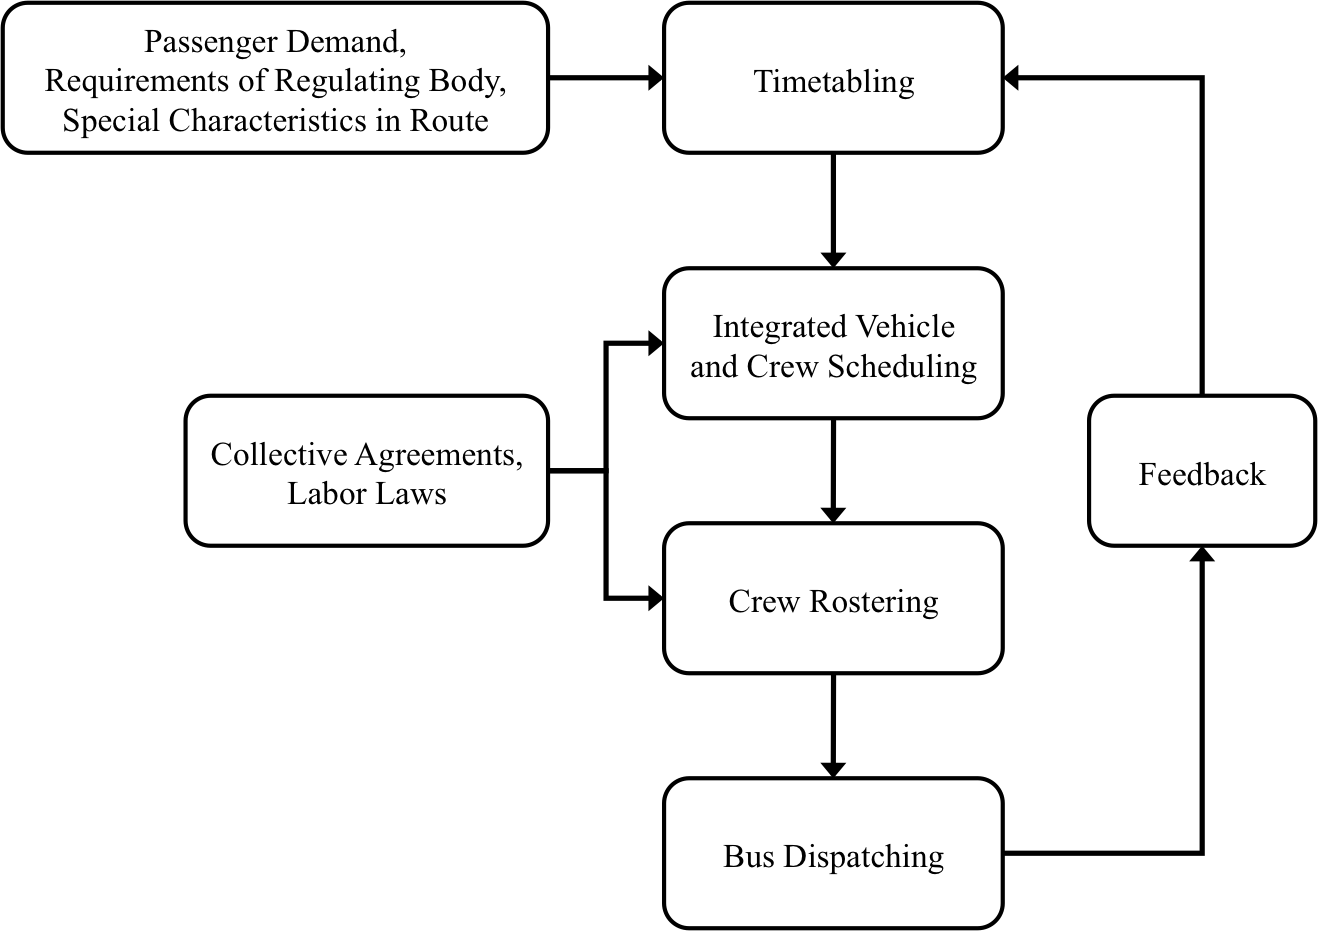
\includegraphics [scale=0.7] {currentBusSchedulingProcess}
\caption[Current Bus Scheduling Process in SL]{Current Bus Scheduling Process in Sri Lanka. Source: \cite{Piyadasa2005}}
\label{image-currentBusSchedulingProcess}
\end{figure}

This process of bus scheduling is an extension of the process put forth by Dennis Huisman in 2004 \cite{Piyadasa2005}. The first step of the process is to conduct a survey. This identifies the existing passenger demand, the quality of the service the buses provide on a given route, the requirements of the regulatory body and any special characteristics of a given route. 

The surveyors ride the buses at variously chosen days and times (to and from the main terminal), note down the trip times and identify the delays and loitering points of the buses on the given route. They also gauge the passenger demand by noting how crowded the bus gets at different stages of the trip. This is a rough estimate of the demand, as the surveyors do not have access to the exact quantitative data.

The next step is the timetable. They formulate this by calculating the average headway for the route. During the formulation of the timetable, the schedulers determine the time the bus service commences and terminates daily for the route. This is done through analyzing the passenger demand data they gather. It is important to correctly identify the time the service commences and terminates daily as it affects the revenue gained by the bus operators and may lead to the operators being unhappy with the timetable. If the service starts too early in the morning or ends too late at night the operators will run at a loss and will not be able to provide a proper service.

Next is the scheduling of the buses to the timetable. The scheduling officers schedule the buses to the bus routes manually using their observations, experience and knowledge. Once the scheduling is complete, the crew rosters are formulated using the schedules. 

Finally, the revised schedule is placed into circulation and used on the bus route (Source: Data gathered through interviews with the Scheduling Unit of the WP RPTA).

As the crew of a particular bus only operates that bus, the steps of vehicle scheduling and crew scheduling could be and should be carried out together. This is known as Integrated Vehicle and Crew Scheduling and literature to support this has been mentioned in the Literature Review of this thesis document.

As mentioned previously, until the mid-2000's the private buses in the Western Province did not have predefined schedules to operate with. The buses were dispatched as soon as they came in to the terminal and the operators did not have predefined working hours and trips to complete for each working day \cite{Piyadasa2005}. However, thanks to research efforts by the University of Moratuwa almost all of the 450+ routes in the Western Province now have working timetables. Despite these timetables being implemented and in operation, they are not being properly adhered to and the quality of the bus service is still well below what is needed.

The bus schedules that are currently in operation take into account both the Economic and Financial cost of the service to the country, the commuters and the bus operators and optimizes the dispatching of the buses via optimal headway manipulation \cite{Piyadasa2005}. After doing numerous mathematical calculations, the methodology identifies the optimal average headway for the route. After identifying the headway, the available buses are scheduled to fill up the timetable as optimally as possible.

A software system was developed to be used to calculate the headways. Ironically however, the system is not being used by the WP RPTA to which it was developed. Instead they use a manual method of determining headway. The NTC however, uses the system to schedule the inter-provincial bus system (data gathered through interviews with Mr. Anuradha Piyadasa, the researcher and developer of the software system).

On inquiry from the personnel at the Scheduling Unit of the WP RPTA, they said that a common observation was that there is a plethora of buses for many of the bus routes in the province, which leads to scheduling difficulties for the Authority. This is due to previous regimes simply doing surveys on the bus service and adding additional buses to the roads, regardless of the requirement. Bus route permits have been issued in mass numbers as a stop-gap solution to the ailing bus service without accounting for the effect it will have on the system as well as the traffic situation. This leads to the revenue gained by each individual bus gradually decreasing (The number of passengers aka the demand stays fairly constant while the number of buses increases which means there are more buses to share in the same revenue. This means that the revenue gained by each individual bus decreases). This has and continues to hinder any efforts for proper reform, restructuring and reengineering of the private bus service in the country.

The timetables that have been implemented currently have research backing them but the bus operators have found numerous ways to circumvent the objectives of these schedules which is to ensure a timely and efficient bus service. This became clearly evident during discussions with the Scheduling Unit of the WP RPTA and from the constant dissatisfaction by the commuters. The bus operators consistently look to maximize their profits with a disregard for the level of service offered to the passenger. The timekeepers and Officers-In-Charge at bus terminals also add to the problem by accepting bribes and neglecting their duties.

Obvious solutions to these problems would be to reduce the trip times in the schedules even more and implement tougher regulations. However, trip times can only be reduced up to a certain point before they become impracticable. The Scheduling Unit is revising the schedules at the moment but it is moving at a snail's pace, not unlike the buses they schedule. 

Also of note is how the revision process is handled. A revision to an existing schedule is not done unless and until sufficient complaints are received from the commuters. One would then think that there was a reasonably efficient complaint process and system in place but this is not so. The complaint mechanism is non-structured which leads to a perfect storm of problems. The commuters are not made aware of the complaint mechanism (no proper channel of disseminating information to the public by way of website/mobile app etc) and complaints are not received, documented and acted upon in a proper fashion (At times only the security guard at the scheduling unit is available to answer the phone and take down complaints when they are received) leading to the status quo continuing. (Source: Discussions with the Scheduling Personnel at the WP RPTA)

\section{Decision Support Systems: an Introduction}
\label{section-DSSIntro}

\paragraph{} According to the nature of the problems currently in the Transportation Service, it is evident that some form of Information System is required to properly manage and monitor it. A Decision Support System seems to suit the need of the transportation service. Therefore, a brief introduction to the concept is provided herewith.

Decision Support Systems are defined as a set of related computer programs and the data required to assist with analysis and decision-making within an organization. The emphasis in DSSs are towards the assistance they provide for the decision-making process. Further details about the idea of DSSs are presented in Section~\ref{section-DSS}.

The requirements of the Transportation Service are such that it suits the offering that DSSs provide. A mechanism that aids the Schedulers in their timetabling process workflow while providing Commuters with the necessary information about the Transportation Service that helps them arrive at an informed decision is exactly what is required. Furthermore, the system's requirements go beyond a simple Management Information System or a Standalone software solution. 

According to \cite{Fedra2000}, in a real-world scenario, a typical decision-making process involves the following characteristics,

\begin {itemize}
\item Multiple actors
\item Conflicting objectives
\item Multiple criteria
\item Plural rationalities
\item Hidden agenda
\end {itemize}

These are consequently exactly what is prevalent in the current Transportation Service in Sri Lanka. \cite{Fedra2000} also presents the following components as included in a general DSS architecture.

\begin {itemize}
\item Information resources
\item The analytical engine
\item The user interface
\end {itemize}

Therefore, it is clear that a DSS is the most suitable Information Systems solution for this type of problem. Later on, in Section~\ref{section-Alternatives}, a more thorough justification will be provided for choosing this type of solution.

\section{Research Goals \& Objectives}
\label{section-ResearchGoalsAndObjectives}

\paragraph{ } Of the problems mentioned in Section~\ref{section-ExistingProblems}, implementing a better bus schedule could solve the first 3. The problem of overcrowded buses could also logically be solved through implementing an effective and efficient timetable. Therefore, this research project focuses on finding a solution to these 4 issues as they are the main and most commonly brought up by the commuters.

We can identify the main goal of the research project as the identification of an Information Systems Solution that assists the Schedulers of the Transport Authority while also providing information to the Commuters to help their decision-making process. 

The Schedulers main business process is the formulation of timetables and schedules and thus addressing it is a core requirement. On the other hand, Commuters need to have Information about the Bus Transportation Service on demand so that they can decide which routes to take, which buses to avoid etc. These two parties also need to be connected in the process of Service Feedback so that the Schedulers are provided with an indication of the level of Service provided by the bus operators. This would lead to a more efficient passenger transport service and will improve commuter satisfaction and productivity.

\section{Research Scope \& Limitations}
\label{section-ResearchScope}

\paragraph{ } The research focuses on finding a DSS-like solution to solve the problems of timetabling, scheduling and information availability. Improving the Schedules and providing a method for commuters to give feedback is what the research project strives to achieve. By achieving this, the bus transport service is improved and made more efficient and reliable. 

The research analyzes how a DSS could be applied to the domain of public transportation in a developing nation. The project then attempted to evaluate the hypothesis by testing it on a group of users. Data was collected via a quantitative survey for the Commuters as well as a qualitative analysis for the Bus Schedulers in the Transport Authority.

The data gathering and automated data collection aspects of the schedulers business process is not within the scope of this research. This project assumes that the data is available already and its integrity and validity is intact.

The research also does not attempt to provide or test any hypothesis related to the application of an Expert System-like solution. The project will limit itself to understanding the IS requirements of the domain and attempting to provide a DSS-like solution to the existing problems.

\section{Outline of Thesis}
\label{section-OutlineOfThesis}

Beyond this point, the thesis document will be structured as follows. Chapter~\ref{chapter-LitReview} will provide a comprehensive review of the literature regarding the planning process of a typical public transportation system. The Chapter also provides an overview of the literature related to Decision Support Systems and gives the reader a look at the concept of DSSs. The Section will also touch on the history and evolution of the DSS concept. The Chapter ends with a brief look at some Information Systems related to transportation services in a few other developing countries.

Chapter~\ref{chapter-ResearchMethodology} will discuss the research methodology followed in this project. It details the steps taken in the research process and identifies possible alternatives for the research problem. The Chapter will also provide information on a Pilot Route Survey that was conducted to gauge the requirements of the system and the shortcomings of the transportation service.

The details of the Proposed Solution will be provided in Chapter~\ref{chapter-ProposedSolution}. the Chapter will detail all the functionality as well as give the reader an overview of the entities in the proposed system. it will end by providing some UI screenshots of the prototype system.

Chapter~\ref{chapter-ResearchEvaluation} will detail the steps taken in the Evaluation phase of the research. the steps taken to evaluate the concept as well as the survey results will be noted in this chapter.

Finally in Chapter~\ref{chapter-ConclusionAndFutureWork}, the conclusions of this research project will be provided and possible future work will be discussed.